\section{Experiments}
\label{Experiment}

\begin{table*}[t]
\begin{center}
\renewcommand{\arraystretch}{1}
\caption{Test accuracy on the CIFAR-10\ /\ 100 dataset. We fix the total client $C=100$ and $P=10$ under training local 50 iterations. We test 3 setups of IID, Dir-1.0, and Dir-0.1 on each dataset. Each group is tested on LeNet~(upper portion) and ResNet-18~(lower portion) models. Each results are tested with 4 different random seeds. ``$-$'' means can not stably converge. ``Family'' distinguishes whether the algorithm is a primal method~(P) or a primal dual method~(PD) and ``Local Opt'' distinguishes whether the algorithm adopts SGD-based or SAM-based local optimizer.}
\vspace{0.1cm}
\scalebox{0.8}{
\begin{sc}
\small
\setlength{\tabcolsep}{2.5mm}{\begin{tabular}{@{}c|cc|cccccc@{}}
\toprule
\multicolumn{1}{c}{\multirow{3}{*}{}} & \multicolumn{1}{c}{\multirow{3}{*}{}} & \multicolumn{1}{c}{\multirow{3}{*}{}} & \multicolumn{3}{c}{CIFAR-10} & \multicolumn{3}{c}{CIFAR-100} \\
\cmidrule(lr){4-6} \cmidrule(lr){7-9}
\multicolumn{1}{c}{} & \multicolumn{1}{c}{Family} & \multicolumn{1}{c}{Local Opt} & \multicolumn{1}{c}{IID} & \multicolumn{1}{c}{Dir-1.0} & \multicolumn{1}{c}{Dir-0.1} & \multicolumn{1}{c}{IID} & \multicolumn{1}{c}{Dir-1.0} & \multicolumn{1}{c}{Dir-0.1} \\
\cmidrule(lr){1-1} \cmidrule(lr){2-9}
FedAvg       & P & SGD & $\text{81.87}_{\pm.12}$ & $\text{80.58}_{\pm.15}$ & $\text{75.57}_{\pm.27}$ & $\text{40.11}_{\pm.17}$ & $\text{39.65}_{\pm.07}$ & $\text{38.37}_{\pm.14}$ \\ 
FedCM        & P & SGD & $\text{80.34}_{\pm.14}$ & $\text{79.31}_{\pm.33}$ & $\text{72.89}_{\pm.37}$ & $\text{43.33}_{\pm.13}$ & $\text{42.35}_{\pm.25}$ & $\text{37.11}_{\pm.51}$ \\ 
SCAFFOLD     & P & SGD & $\text{84.25}_{\pm.16}$ & $\text{83.61}_{\pm.14}$ & $\text{78.66}_{\pm.29}$ & $\text{49.65}_{\pm.06}$ & $\text{49.11}_{\pm.14}$ & $\text{46.36}_{\pm.30}$ \\ 
FedSAM       & P & SAM & $\text{83.22}_{\pm.09}$ & $\text{81.94}_{\pm.13}$ & $\text{77.41}_{\pm.36}$ & $\text{43.02}_{\pm.09}$ & $\text{42.83}_{\pm.29}$ & $\text{42.29}_{\pm.23}$ \\  
FedDyn       & PD & SGD & $\text{84.49}_{\pm.22}$ & $\text{84.20}_{\pm.14}$ & $\text{79.51}_{\pm.13}$ & $\text{50.27}_{\pm.11}$ & $\text{49.64}_{\pm.21}$ & $\text{46.30}_{\pm.26}$ \\ 
FedSpeed     & PD & SAM & $\text{86.01}_{\pm.18}$ & $\text{85.11}_{\pm.21}$ & $\text{80.86}_{\pm.18}$ & $\text{54.01}_{\pm.15}$ & $\text{53.45}_{\pm.23}$ & $\text{51.28}_{\pm.18}$ \\
\cmidrule(lr){1-1} \cmidrule(lr){2-9}
A-FedPD      & PD & SGD & $\text{85.31}_{\pm.14}$ & $\text{84.94}_{\pm.13}$ & $\text{80.28}_{\pm.20}$ & $\text{51.41}_{\pm.15}$ & $\text{51.17}_{\pm.17}$ & $\text{48.15}_{\pm.28}$ \\  
A-FedPDSAM   & PD & SAM & $\textbf{86.47}_{\pm.18}$ & $\textbf{85.90}_{\pm.29}$ & $\textbf{81.96}_{\pm.19}$ & $\textbf{55.56}_{\pm.27}$ & $\textbf{54.62}_{\pm.16}$ & $\textbf{53.15}_{\pm.19}$ \\  
\cmidrule(lr){1-1} \cmidrule(lr){2-9}
FedAvg       & P & SGD & $\text{81.67}_{\pm.21}$ & $\text{80.94}_{\pm.17}$ & $\text{76.24}_{\pm.35}$ & $\text{44.68}_{\pm.21}$ & $\text{44.27}_{\pm.25}$ & $\text{41.64}_{\pm.27}$ \\ 
FedCM        & P & SGD & $\text{84.22}_{\pm.17}$ & $\text{82.85}_{\pm.21}$ & $\text{76.93}_{\pm.32}$ & $\text{50.04}_{\pm.16}$ & $\text{48.66}_{\pm.28}$ & $\text{44.07}_{\pm.30}$ \\ 
SCAFFOLD     & P & SGD & $\text{84.31}_{\pm.14}$ & $\text{83.70}_{\pm.11}$ & $\text{78.70}_{\pm.21}$ & $\text{50.69}_{\pm.21}$ & $\text{50.28}_{\pm.21}$ & $\text{47.12}_{\pm.34}$ \\ 
FedSAM       & P & SAM & $\text{83.79}_{\pm.28}$ & $\text{82.58}_{\pm.19}$ & $\text{77.83}_{\pm.27}$ & $\text{48.66}_{\pm.29}$ & $\text{48.42}_{\pm.19}$ & $\text{45.03}_{\pm.22}$ \\  
FedDyn       & PD & SGD & $\text{83.71}_{\pm.26}$ & $\text{82.66}_{\pm.15}$ & $\text{79.44}_{\pm.25}$ & $-$ & $-$ & $-$ \\ 
FedSpeed     & PD & SAM & $\text{86.90}_{\pm.18}$ & $\text{85.92}_{\pm.24}$ & $\text{81.47}_{\pm.19}$ & $\text{53.22}_{\pm.28}$ & $\text{52.75}_{\pm.16}$ & $\text{49.66}_{\pm.13}$ \\
\cmidrule(lr){1-1} \cmidrule(lr){2-9}
A-FedPD      & PD & SGD & $\text{85.11}_{\pm.12}$ & $\text{84.33}_{\pm.16}$ & $\text{81.05}_{\pm.28}$ & $\text{48.15}_{\pm.22}$ & $\text{48.02}_{\pm.29}$ & $\text{46.24}_{\pm.26}$ \\  
A-FedPDSAM   & PD & SAM & $\textbf{87.44}_{\pm.13}$ & $\textbf{86.46}_{\pm.25}$ & $\textbf{82.48}_{\pm.21}$ & $\textbf{55.30}_{\pm.23}$ & $\textbf{53.49}_{\pm.17}$ & $\textbf{50.31}_{\pm.23}$ \\  
\bottomrule
\end{tabular}}
\label{acc}
\end{sc}
}
\end{center}
\vspace{-0.4cm}
\end{table*}

In this section, we introduce the experiments conducted to validate the efficiency of our proposed \textit{A-FedPD} and a variant \textit{A-FedPDSAM}~(see details in Appendix~\ref{ap:fedpdsam}). We first introduce experimental setups and benchmarks, and then we show the empirical studies. 

% \subsection{Setups}
% \label{setups}

\textbf{Backbones and Datasets.} In our experiments, we adopt LeNet~\cite{lecun1998gradient} and ResNet~\cite{he2016deep} as backbones. We follow previous work to test the performance of benchmarks on the CIFAR-10\ /\ 100 dataset~\cite{krizhevsky2009learning}. We introduce the heterogeneity to split the raw dataset to local clients with independent Dirichlet distribution~\cite{hsu2019measuring} controlled by a concentration parameter. In our setups, we mainly test the performance of the IID, Dir-1.0, and Dir-0.1 splitting. The Dir-1.0 represents the low heterogeneity and Dir-0.1 represents the high heterogeneity. We also adopt the sampling with replacement to further enhance the heterogeneity.

\textbf{Setups.} We test the accuracy experiments on $C=100$ and $P/C=10\%$, which is also the most popular setup in the FL community. In the comparison experiments, we test the participated ratio $P/C=\left[5\%,10\%,20\%,50\%,80\%,100\%\right]$ and local interval $K=\left[10,20,50,100,200\right]$ respectively. In each setup, for a fair comparison, we freeze the most of hyperparameters for all methods. We fix total communication rounds $T=800$ except for the ablation studies.
%The detailed hyperparameter selections are stated in Appendix~\ref{}.

\textbf{Baselines.} \textit{FedAvg}~\citep{mcmahan2017communication} is the fundamental paradigm in FL scenarios. \textit{FedCM}~\citep{xu2021fedcm}, \textit{SCAFFOLD}~\citep{karimireddy2020scaffold} and \textit{FedSAM}~\citep{qu2022generalized} are three classical SOTA methods in the federated primal average family. \textit{FedDyn}~\citep{durmus2021federated} and \textit{FedSpeed}~\cite{sun2023fedspeed} are relatively stable federated primal dual methods. A more detailed introduction of these methods is presented in Table~\ref{acc}, including the family-basis and local optimizer.

\subsection{Experiments}
\label{experiments}

In this part, we introduce the phenomena observed in our empirical studies. We primarily investigated performance comparisons, including settings with different participation rates, various local intervals, and different numbers of communication rounds. Then we report the comparison of wall-clock time.

\textbf{Performance Comparison.} Table~\ref{acc} shows the test accuracy on CIFAR-10\ /\ 100 dataset. The vanilla \textit{FedAvg} provides the standard bars as the baseline. In the \textit{federated primal average} methods, The \textit{FedCM} is not stable enough and is largely affected by different backbones, which is caused by the forced consistency momentum and may introduce very large biases. \textit{SCAFFOLD} and \textit{FedSAM} performs well. However, both are less than the \textit{primal dual}-based methods. In summary, \textit{SCAFFOLD} is on average 3.2\% lower than \textit{FedSpeed}. As heterogeneity increases, \textit{SCAFFOLD} drops on average about 5.6\% on CIFAR-10 and 3.43\% on CIFAR-100. In the \textit{federated primal dual} methods, we can clearly see that \textit{FedDyn} is not stable in the training. It performs well on the LeNet, which could achieve at least 1\% improvements than \textit{SCAFFOLD}. However, when the task becomes difficult, i.e., ResNet-18 on CIFAR-100, its accuracy is affected by the ``dual drift'' and drops quickly. To maintain stability, we have to select some weak coefficients to stabilize it and finally get a lower accuracy. Our proposed \textit{A-FedPD} could efficiently alleviate the negative impacts of the ``dual drift''. It performs about on average 0.8\% higher than \textit{FedDyn} on the CIFAR-10 dataset. When \textit{FedDyn} has to compromise the hyperparameters and becomes extremely unstable on ResNet-18 on the CIFAR-100 dataset, \textit{A-FedPD} still performs stably. It's also very scalable. When we introduce the \textit{SAM} optimizer to replace the vanilla \textit{SGD}, it could achieve higher performance.

\begin{figure*}[t]
\vskip -0.05in
\centering
    \subfigure[Different Participation Ratios.]{
	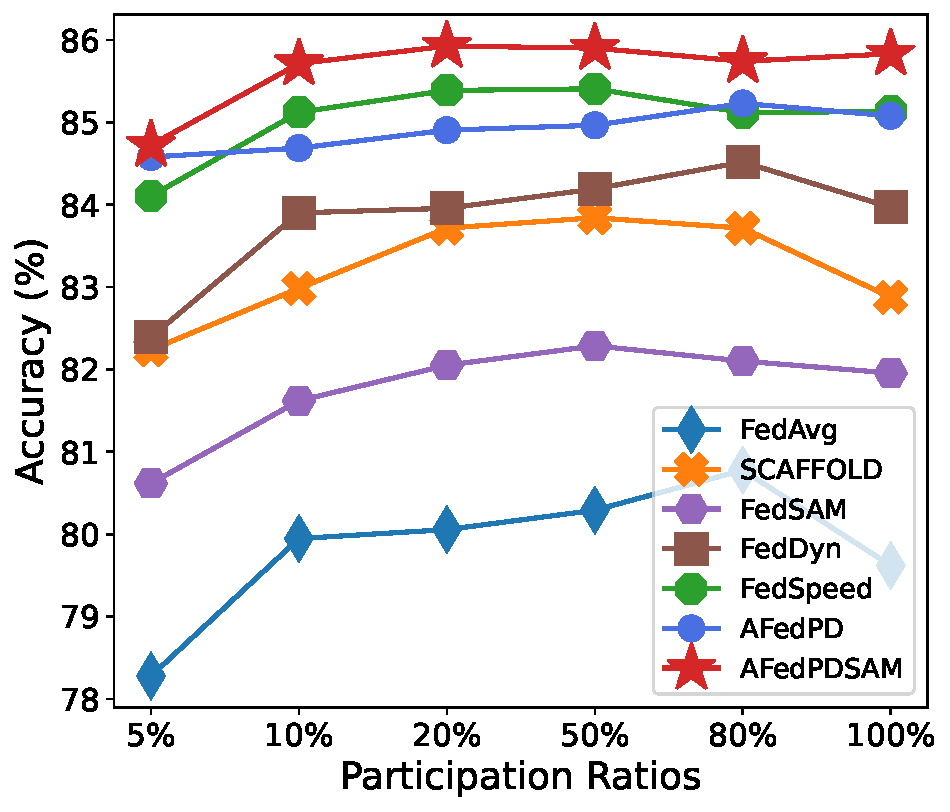
\includegraphics[width=0.33\textwidth]{figure/ab_different_active.pdf}}\!\!\!
    \subfigure[Different Local Intervals.]{
        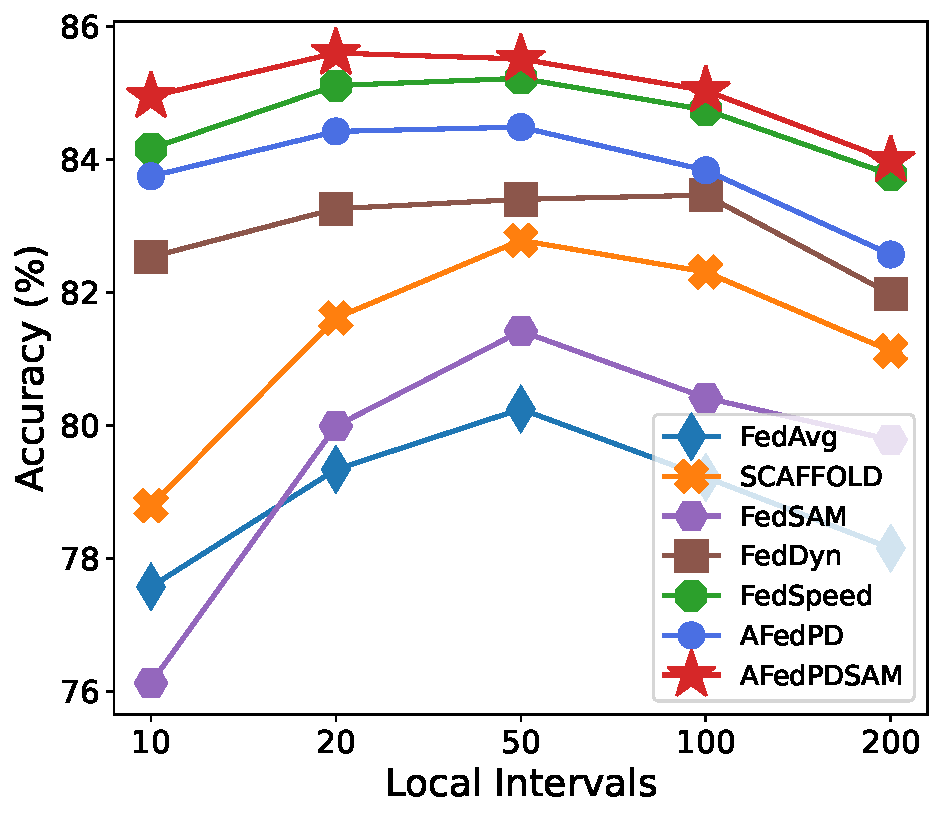
\includegraphics[width=0.33\textwidth]{figure/ab_different_interval.pdf}}\!\!\!
    \subfigure[Different Rounds.]{
	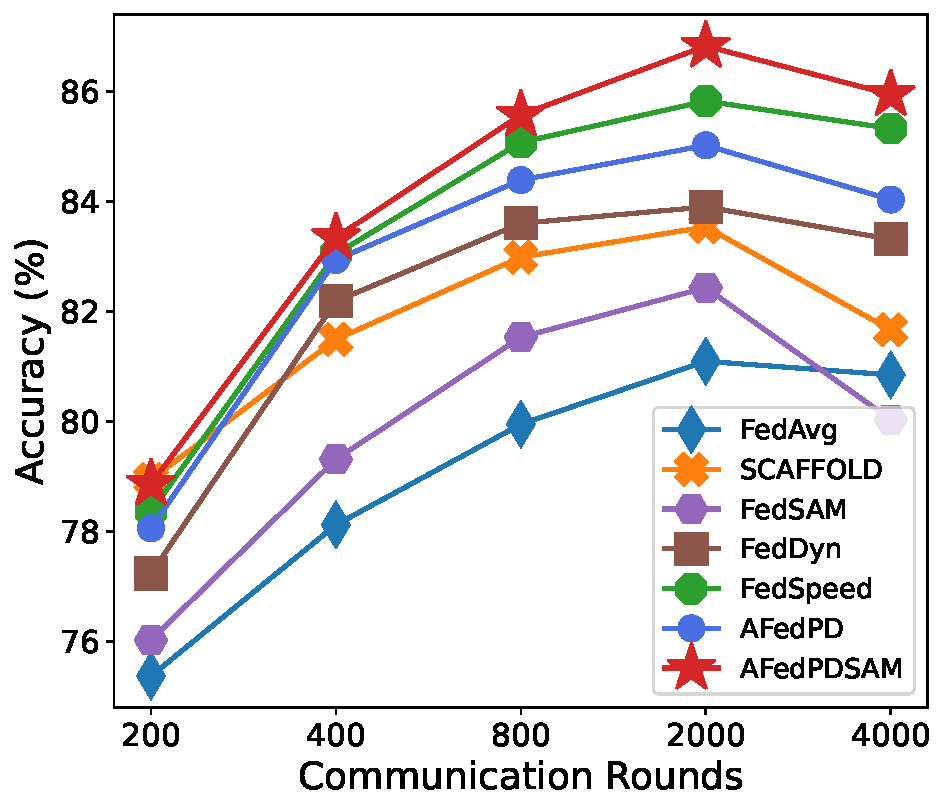
\includegraphics[width=0.33\textwidth]{figure/ab_different_round.pdf}}
\vskip -0.1in
\caption{Test of the proposed \textit{A-FedPD} method on setups of different participation ratios, different local intervals, and different rounds. In these experiments, we fix the total training data samples and total training iterations and then learn their variation trends.}
\label{ablations}
\vskip -0.15in
\end{figure*}

\textbf{Different Participation Ratios.} In this part we compare the sensitivity to the participation ratios. In each setup, we fix the scale as 100 and the local interval as 50 iterations. Active ratio is selected from $\left[5\%, 10\%, 20\%, 50\%, 80\%, 100\%\right]$ as shown in Figure~\ref{ablations} (a). Under frozen hyperparameters, all methods perform well on each selection. The best performance is approximately located in the range of $[20\%, 80\%]$. Our proposed methods achieve high efficiency in handling large-scale training, which performs more steadily than other benchmarks across all selections.

\textbf{Different Local Intervals.} In this part we compare the sensitivity to the local intervals. In each setup, we fix the scale as 100 and the participation as 10\%. Local interval $K$ is selected from $\left[10, 20, 50, 100, 200\right]$ as shown in Figure~\ref{ablations} (b). More local training iterations usually mean more overfitting on the local dataset, which leads to a serious ``client drift'' issue. All methods will be affected by this and drop accuracy. It is a trade-off in selecting the local interval $K$ to balance both optimization efficiency and generalization stability. Our proposed methods still could achieve the best performance even on the very long local training iterations.

\textbf{Different Communication Rounds.} In this part, we compare the sensitivity to the communication rounds. In each setup, we fix total iterations $TK = 40,000$. Communication round $T$ is selected from $\left[200, 400, 800, 2000, 4000\right]$ as shown in Figure~\ref{ablations} (c). We always expect the local clients can handle more and communicate less, which will significantly reduce the communication costs. In the experiments, our proposed methods could achieve higher efficiency than the benchmarks. \textit{A-FedPD} saves about half the communication overhead compared to \textit{SCAFFOLD}, and about one-third of \textit{FedDyn}. Under favorable communication bandwidths, they can achieve SOTA performance.

\begin{wrapfigure}[13]{r}{0.5\textwidth}
\centering
\vspace{-0.6cm}
    \subfigure[ResNet-18.]{
        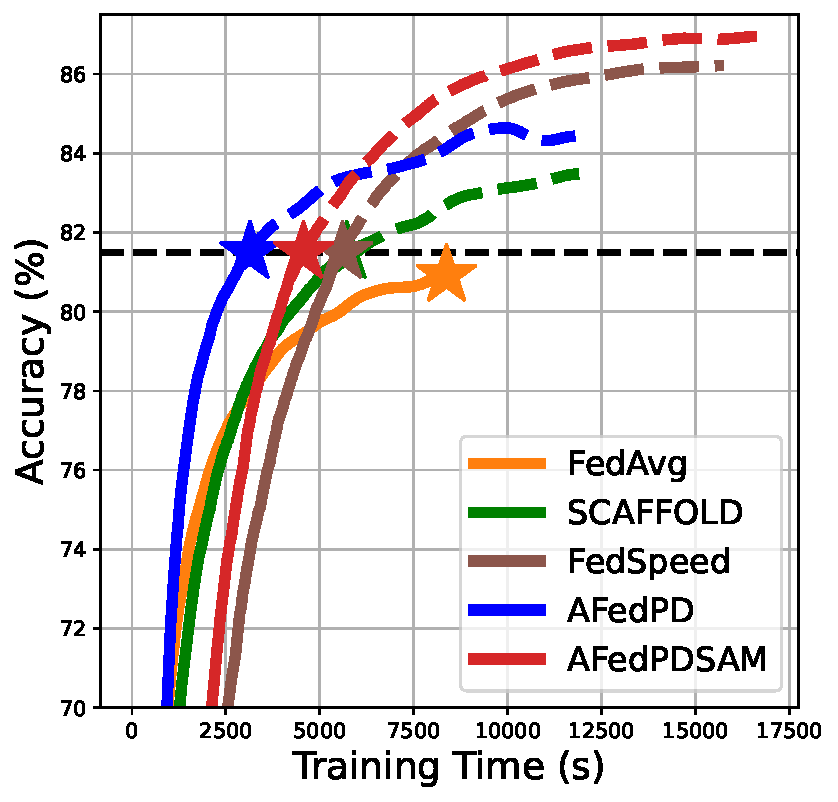
\includegraphics[width=0.249\textwidth]{figure/wall_clock_time_resnet.pdf}}\!\!\!
    \subfigure[LeNet.]{
	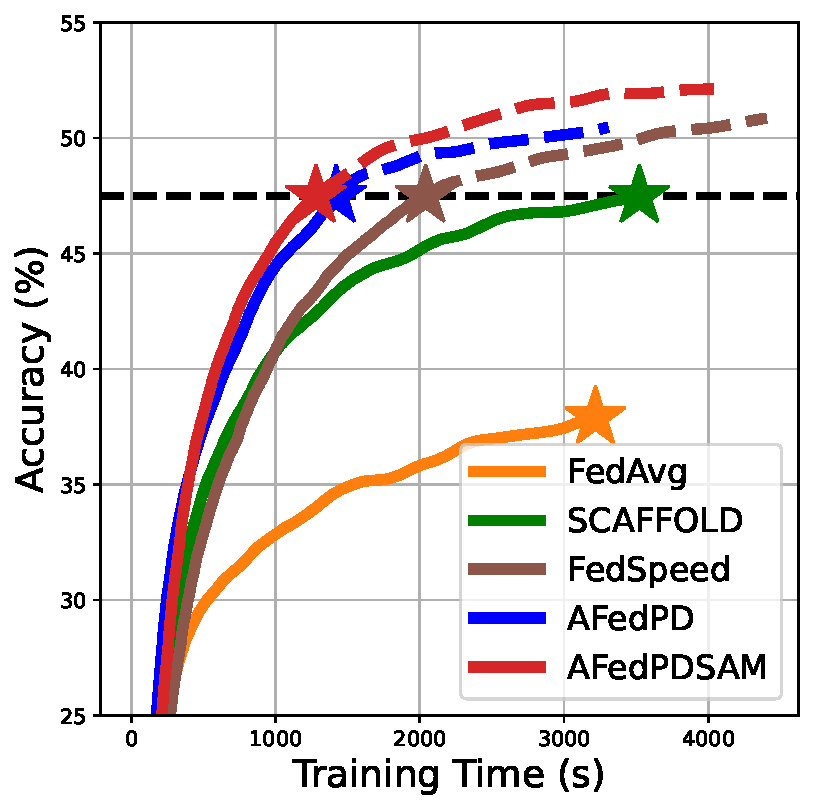
\includegraphics[width=0.243\textwidth]{figure/wall_clock_time_cifar100.pdf}}
 \vskip -0.1in
\caption{Wall-clock time test of training process after total of 600 communication rounds.}
\label{wall clock time}
 \vskip -0.1in
\end{wrapfigure}

\textbf{Wall-clock Time Efficiency.} In this part we test the practical wall-clock time comparisons as shown in Figure~\ref{wall clock time}. Though some methods are communication-efficiency, complicated calculations hinder the real efficiency in wall-clock training time. Though \textit{FedSpeed} and \textit{AFedPDSAM} perform well at the end, additional calculations per single round make their early-stage competitiveness lower. \textit{AFedPD} and \textit{SCAFFOLD} consume fewer time costs, hence achieving better results at the early stage. Without considering training time costs, \textit{AFedPDSAM} achieves the SOTA results at the end. Detailed comparisons are stated in Sec.\ref{wall=clock}.